\documentclass[11pt]{article}
\usepackage[utf8]{inputenc}	% Para caracteres en español
\usepackage{amsmath,amsthm,amsfonts,amssymb,amscd}
\usepackage{multirow,booktabs}
\usepackage[table]{xcolor}
\usepackage{fullpage}
\usepackage{lastpage}
\usepackage{enumitem}
\usepackage{fancyhdr}
\usepackage{mathrsfs}
\usepackage{wrapfig}
\usepackage{setspace}
\usepackage{calc}
\usepackage{multicol}
\usepackage{cancel}
\usepackage{float}
\usepackage{physics}
\usepackage[retainorgcmds]{IEEEtrantools}
\usepackage[margin=1cm]{geometry}
\usepackage{amsmath}
\newlength{\tabcont}
\setlength{\parindent}{0.0in}
\setlength{\parskip}{0.05in}
\usepackage{empheq}
\usepackage{framed}
\usepackage[most]{tcolorbox}
\usepackage{xcolor}
\usepackage[version=3]{mhchem}
\usepackage[english]{babel}
\usepackage[utf8]{inputenc}
\usepackage{graphicx}
\usepackage[colorinlistoftodos]{todonotes}

\colorlet{shadecolor}{orange!15}
\parindent 0in
\parskip 12pt
\geometry{margin=1in, headsep=0.25in}
\theoremstyle{definition}
\newtheorem{defn}{Definition}
\newtheorem{reg}{Rule}
\newtheorem{exer}{Exercise}
\newtheorem{note}{Note}
\begin{document}
\setcounter{section}{2}
%\setcounter{subsection}{}
\title{Problem Set 5}

%==============================================================
%\thispagestyle{empty}
\pagestyle{fancy}
\fancyhf{}
\rhead{Physics 180}
\chead{Problem Set 5}
\lhead{Olyn D. Desabelle}
\rfoot{Page \thepage}

\begin{center}
{\LARGE \bf Problem Set 5}\\
%{\large Physics 180}\\
%Olyn D. Desabelle
\end{center}

\begin{figure}[h!]
    \centering
    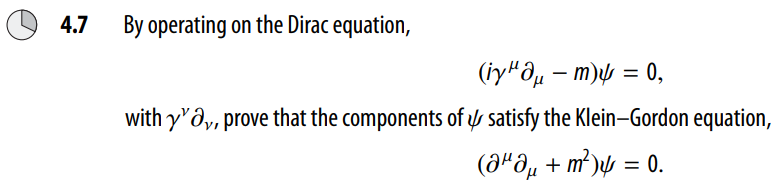
\includegraphics[scale = 0.5]{4.7.png}
\end{figure}

We start with the given equation:

\begin{align*}
    (i \gamma^{\mu} \partial_{\mu} - m)\psi = 0
\end{align*}

operating on it with $\gamma^{\nu} \partial_{\nu}$, we get:

\begin{align*}
    \gamma^{\nu} \partial_{\nu} \left[ (i \gamma^{\mu} \partial_{\mu} - m)\psi = 0 \right]\\
    (i \gamma^{\nu}\gamma^{\mu} \partial_{\nu}\partial_{\mu} - m\gamma^{\nu} \partial_{\nu})\psi = 0
\end{align*}

we can operate on this with $-i$ to get:

\begin{align*}
   -i \left[(i \gamma^{\nu}\gamma^{\mu} \partial_{\nu}\partial_{\mu} - m\gamma^{\nu} \partial_{\nu})\psi = 0\right]\\
    (\gamma^{\nu}\gamma^{\mu} \partial_{\nu}\partial_{\mu} +i m\gamma^{\nu} \partial_{\nu})\psi = 0
\end{align*}

we note that the wavefunction satisfies the Dirac equation (Eqn. 4.39) $(i \gamma^{\mu}\partial_{\mu} - m)\psi = 0$:

\begin{align*}
    i \gamma^{\nu}\partial_{\nu}\psi = m\psi
\end{align*}

we can use this with our original equation:

\begin{align*}
    (\gamma^{\nu}\gamma^{\mu} \partial_{\nu}\partial_{\mu} +m[i\gamma^{\nu} \partial_{\nu}])\psi = 0\\
    (\gamma^{\nu}\gamma^{\mu} \partial_{\nu}\partial_{\mu} + m^2)\psi = 0
\end{align*}

we note that this holds true even if we switch indices:

\begin{align*}
    (\gamma^{\mu}\gamma^{\nu} \partial_{\mu}\partial_{\nu} + m^2)\psi = 0
\end{align*}

adding these two, we get:

\begin{align*}
    (\gamma^{\nu}\gamma^{\mu} \partial_{\nu}\partial_{\mu} + m^2)\psi + (\gamma^{\mu}\gamma^{\nu} \partial_{\mu}\partial_{\nu} + m^2)\psi = 0 \\
    (\left[\gamma^{\nu}\gamma^{\mu} \partial_{\nu}\partial_{\mu} + \gamma^{\mu}\gamma^{\nu}\partial_{\mu}\partial_{\nu}\right] + 2m^2)\psi =0\\
    \left( \frac{1}{2}\left[\gamma^{\nu}\gamma^{\mu} \partial_{\nu}\partial_{\mu} + \gamma^{\mu}\gamma^{\nu}\partial_{\mu}\partial_{\nu}\right] + m^2 \right)\psi =0
\end{align*}

we note that we can switch up the order of differentiation in the second term in brackets:

\begin{align*}
    \frac{1}{2}\left[\gamma^{\nu}\gamma^{\mu} \partial_{\nu}\partial_{\mu} + \gamma^{\mu}\gamma^{\nu}\partial_{\mu}\partial_{\nu}\right] = 
    \frac{1}{2}\left[\gamma^{\nu}\gamma^{\mu} \partial_{\nu}\partial_{\mu} + \gamma^{\mu}\gamma^{\nu}\partial_{\nu}\partial_{\mu}\right]\\
    \frac{1}{2}\left[\gamma^{\nu}\gamma^{\mu} \partial_{\nu}\partial_{\mu} + \gamma^{\mu}\gamma^{\nu}\partial_{\mu}\partial_{\nu}\right]=  
    \frac{1}{2}\left[\gamma^{\nu}\gamma^{\mu}  + \gamma^{\mu}\gamma^{\nu}\right]\partial_{\nu}\partial_{\mu}
\end{align*}

our original equation becomes:

\begin{align*}
    \left(  \frac{1}{2}\left[\gamma^{\nu}\gamma^{\mu}  + \gamma^{\mu}\gamma^{\nu}\right]\partial_{\nu}\partial_{\mu} + m^2 \right)\psi =0
\end{align*}

we note of the anticommutation relation (Eqn. 4.33) $\gamma^{\nu}\gamma^{\mu}  + \gamma^{\mu}\gamma^{\nu} = 2g^{\mu\nu}$:

\begin{align*}
    \frac{1}{2}\left[\gamma^{\nu}\gamma^{\mu}  + \gamma^{\mu}\gamma^{\nu}\right]\partial_{\nu}\partial_{\mu}=  
    g^{\mu\nu}\partial_{\nu}\partial_{\mu}
\end{align*}

then we get:

\begin{align*}
    \left(  g^{\mu\nu}\partial_{\nu}\partial_{\mu} + m^2 \right)\psi =0
\end{align*}

we note that we can rewrite $g^{\mu\nu}\partial_{\nu}\partial_{\mu}$ as:

\begin{align*}
    g^{\mu\nu}\partial_{\nu}\partial_{\mu} = \partial^{\mu} \partial_{\mu}
\end{align*}

thus our original equation becomes the Klein-Gordon equation:

\begin{equation}
\boxed{
    \left(\partial^{\mu} \partial_{\mu} + m^2 \right)\psi =0
}
\end{equation}

%we then note that we can switch up the order of differentiation:

%\begin{align*}
%    \gamma^{\nu}\gamma^{\mu} \partial_{\nu}\partial_{\mu} = \gamma^{\mu}\gamma^{\nu} \partial_{\mu}\partial_{\nu}\\
%    2\gamma^{\nu}\gamma^{\mu} \partial_{\nu}\partial_{\mu} = \gamma^{\mu}\gamma^{\nu} \partial_{\mu}\partial_{\nu} +  \gamma^{\nu}\gamma^{\mu} \partial_{\nu}\partial_{\mu}\\
%\end{align*}


%==============================================================
\newpage
%==============================================================

\begin{figure}[h!]
    \centering
    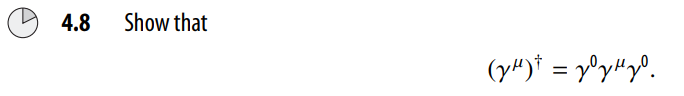
\includegraphics[scale = 0.55]{4.8.png}
\end{figure}

To show that $(\gamma^{\mu})^{\dagger} = \gamma^{0} \gamma^{\mu} \gamma^{0}$, we show that this holds for $\mu=0$ and $\mu= k \neq 0$. \newline

$\underline{\mu=0}$

For $\mu=0$, the LHS of our equation becomes:

\begin{align*}
    \text{LHS: }\; (\gamma^{0})^{\dagger}
\end{align*}

As $\gamma^{0}$ is Hermitian (Eqn. 4.34), then this becomes:

\begin{align*}
    \text{LHS: }\; (\gamma^{0})^{\dagger} = \gamma^{0}
\end{align*}

The original equation becomes:

\begin{align*}
    \gamma^{0} = \gamma^{0}\gamma^{0}\gamma^{0}
\end{align*}

with the $\gamma^{0}$ defined as $\gamma^{0} = \begin{pmatrix}
    I & 0 \\
    0 & -I
\end{pmatrix} = \begin{pmatrix}1&0&0&0\\ 0&1&0&0\\ 0&0&-1&0\\ 0&0&0&-1 \end{pmatrix}$, we evaluate the RHS of the equation:

\begin{align*}
    \text{RHS: }\; \gamma^{0}\gamma^{0}\gamma^{0} = 
    \begin{pmatrix}1&0&0&0\\ 0&1&0&0\\ 0&0&-1&0\\ 0&0&0&-1\end{pmatrix}
    \begin{pmatrix}1&0&0&0\\ 0&1&0&0\\ 0&0&-1&0\\ 0&0&0&-1\end{pmatrix}
    \begin{pmatrix}1&0&0&0\\ 0&1&0&0\\ 0&0&-1&0\\ 0&0&0&-1\end{pmatrix}\\
    \text{RHS: }\; \gamma^{0}\gamma^{0}\gamma^{0} =
    \begin{pmatrix}1&0&0&0\\ 0&1&0&0\\ 0&0&1&0\\ 0&0&0&1\end{pmatrix}
    \begin{pmatrix}1&0&0&0\\ 0&1&0&0\\ 0&0&-1&0\\ 0&0&0&-1\end{pmatrix}\\
    \text{RHS: }\; \gamma^{0}\gamma^{0}\gamma^{0} =
    \begin{pmatrix}1&0&0&0\\ 0&1&0&0\\ 0&0&-1&0\\ 0&0&0&-1\end{pmatrix} = \gamma^{0}
\end{align*}

the RHS = LHS, and thus we now have shown that $(\gamma^{\mu})^{\dagger} = \gamma^{0} \gamma^{\mu} \gamma^{0}$ for $\mu=0$. We proceed with showing this is also true for $\mu=k\neq 0$.\newline


$\underline{\mu=k\neq 0}$

For $\mu=k \neq 0$, the LHS of our equation becomes:

\begin{align*}
    \text{LHS: }\; (\gamma^{k})^{\dagger}
\end{align*}

As $\gamma^{k}$ is anti-Hermitian (Eqn. 4.34), then this becomes:

\begin{align*}
    \text{LHS: }\; (\gamma^{k})^{\dagger} = -\gamma^{k}
\end{align*}

The original equation becomes:

\begin{align*}
    -\gamma^{k} = \gamma^{0}\gamma^{k}\gamma^{0}
\end{align*}

we note that we have the given Dirac-Pauli representation of the $\gamma$-matrices for $k=1,2,3$:

\begin{align*}
    \gamma^{1} = 
    \begin{pmatrix}
        0&0&0&1\\ 
        0&0&1&0\\ 
        0&-1&0&0\\ 
        -1&0&0&0
    \end{pmatrix}\\
    \gamma^{2} = 
    \begin{pmatrix}
        0&0&0&-i\\ 
        0&0&i&0\\ 
        0&i&0&0\\ 
        -i&0&0&0
    \end{pmatrix}\\
    \gamma^{3} = 
    \begin{pmatrix}
        0&0&1&0\\ 
        0&0&0&-1\\ 
        -1&0&0&0\\ 
        0&1&0&0
    \end{pmatrix}
\end{align*}

noting the zeros common with them then in general, we can then express the matrices as:

\begin{align*}
    \gamma^{k} =
    \begin{pmatrix}
        0&0&a&b\\ 
        0&0&c&d\\ 
        f&g&0&0\\ 
        h&j&0&0\end{pmatrix}
\end{align*}

using this, then when we evaluate the RHS of the equation, we get:

\begin{align*}
    \text{RHS: }\; \gamma^{0}\gamma^{k}\gamma^{0}
    =
    \begin{pmatrix}1&0&0&0\\ 0&1&0&0\\ 0&0&-1&0\\ 0&0&0&-1 \end{pmatrix}
    \begin{pmatrix}
        0&0&a&b\\ 
        0&0&c&d\\ 
        f&g&0&0\\ 
        h&j&0&0\end{pmatrix}
    \begin{pmatrix}1&0&0&0\\ 0&1&0&0\\ 0&0&-1&0\\ 0&0&0&-1 \end{pmatrix}\\
    \text{RHS: }\; \gamma^{0}\gamma^{k}\gamma^{0}
    =
    \begin{pmatrix}0&0&a&b\\ 0&0&c&d\\ -f&-g&0&0\\ -h&-j&0&0\end{pmatrix}
    \begin{pmatrix}1&0&0&0\\ 0&1&0&0\\ 0&0&-1&0\\ 0&0&0&-1\end{pmatrix}\\
    \text{RHS: }\; \gamma^{0}\gamma^{k}\gamma^{0}
    =
    \begin{pmatrix}0&0&-a&-b\\ 0&0&-c&-d\\ -f&-g&0&0\\ -h&-j&0&0\end{pmatrix}
    = - \gamma^{k}
\end{align*}

the RHS = LHS, and thus we now have shown that $(\gamma^{\mu})^{\dagger} = \gamma^{0} \gamma^{\mu} \gamma^{0}$ for $\mu=k \neq 0$. Since the conditions have been met for $\mu=0$ and $\mu \neq 0$, then we have shown that in general:

\begin{equation*}
\boxed{
    (\gamma^{\mu})^{\dagger} = \gamma^{0} \gamma^{\mu} \gamma^{0}
}
\end{equation*}

%we note that in our earlier solution evaluating $\gamma^{0}\gamma^{0}\gamma^{0}$, we found that $\gamma^{0}\gamma^{0} = \begin{pmatrix}1&0&0&0\\ 0&1&0&0\\ 0&0&1&0\\ 0&0&0&1\end{pmatrix} = I$. Thus we can rewrite the LHS of the equation as:

%\begin{align*}
%    -\gamma^{k} = -I\gamma^{k}\\
%    -\gamma^{k} = -\gamma^{0}\gamma^{0}\gamma^{k}
%\end{align*}

%we can rewrite the RHS of the equation as:

%\begin{align*}
%    \gamma^{0}\gamma^{k}\gamma^{0} = 
%\end{align*}
%==================================
\end{document}